

\section{Introduction}\label{Introduction}
Globular clusters (\acsp{GC})\acused{GC} are self-gravitating, gas-free systems of 10\(^6\) to 10\(^8\) stars which are spherically grouped. There are about 150 of them in the \ac{MW}. Since they are some of the oldest stellar populations in the universe (approximately 13 Gyr), they contain much information about the assembly history and evolution of the \ac{MW}. Formerly seen as very simple systems with only one stellar population and without rotation recent research revealed a much higher complexity of these systems. \acp{GC} are now know to host multiple stellar populations that challenge our understanding of their formation. Moreover, \acp{GC} now appear dynamically complex, presenting deviations from spherical symmetry, anisotropy in velocity space and significant internal rotation.
 
\par Recent attention has been devoted to the search of \acp{IMBH} in the centre of \acp{GC}. In their centre \acp{GC} could host an \ac{IMBH}. These could be the missing link between stellar mass black holes \color{red} mass \color{black} and \acp{SMBH} \color{red} mass \color{black} as origin of the \ac{SMBH}, expected to have a mass between \(10^3-10^4 \mathrm{M}_\odot\). \par The kinematic detection of \acp{IMBH} is usually based on the analysis of the velocity-dispersion profile in the inner few arcseconds around the crowded centre of a \ac{GC}. This requires a combination of high angular resolution and high spectral resolving power. For this reason the detection of \acp{IMBH} remains highly controversial. Currently there are two different kinematic methods trying to detect \acp{IMBH}: \color{red} resolved kinematics \& unresolved integrated light [bianchini 2015] \color{black} As an example there are the unresolved/integrated IFU kinematics which result in a signature of an \ac{IMBH} for NGC 6388 and resolved/discrete kinematics which do not yield \acp{IMBH}. \color{red} include graph of Paolo's talk!! \color{black} 
\\

%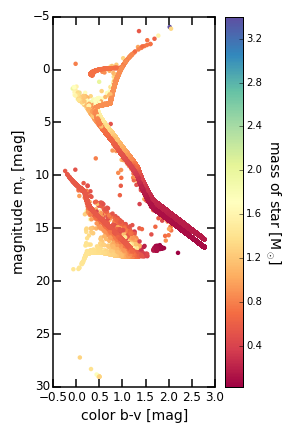
\includegraphics[width=\textwidth]{Plots/color_magnitude_diagram}
%\subsection{Orbits \& actions}
\par An orbit is a path a unperturbed, collisionless tracer particle (e.g. a star) will move along in a gravitational potential. Orbits contain information about the gravitational potential generated by the mass distribution of a system in their position and velocity coordinates following Newtons 2nd law. Orbit \acp{DF} describe which orbits are populated by how many tracers. From the orbit distribution function together with the overall potential we can draw inferences about the structure and evolution history of the system. 
\par Historically observations of orbits enabled discoveries or confirmed them: 
\begin{itemize}
\item Seen from the earth Mars' position moves over the sky as a loop called epicycle. That implies that the earth is not the centre of the universe! (C \& O p.3)
\item Neptune/Uranus \color{red} noch mal nachlesen \color{black}
\item From rotation curves of galaxies we see that stars move faster than what expected by the presence of only the mass of luminous matter. There has to be more matter interacting via gravitational forces. This has led to the theory of dark matter. (Rubin 1980)
\item Mercury's orbit differs hugely from calculated Kepler orbit. This is because of its migrating pericentre. Due to the proximity to the sun gravitational forces are so strong that we need to apply general relativity.
\item The \ac{SMBH} Sagittarius A*  was detected by observations of the orbits around the black hole and resulting mass calculations. (C \& O p.923)
\end{itemize}
\par Some examples for orbit \acp{DF} are spiral galaxies where stars of different components (thin disc, thick disc, bulge, halo) are on different orbits (dynamical distinct) and have different metallicities (chemical distinct).
\\\par Actions are integrals of motion and are the distinct description of orbits. They are constant with time. Known for a long time they are extremly difficult to calculate. Actions of our solar system can be calculated easier since the potential is a Kepler potential. With nowadays supercomputers it is finally possible to compute actions of more complex and less explored systems.
\color{green} how to describe orbits \\ idea 1 (x(t),v(t)) pretty complicated time evolution in 6 coordinates. idea 2 take quantities which are constant with time so called integrals of motions \\ beste set von integrals of motions are actions good to interpret \color{black}
\\\par We propose to explore a new method to test if we can predict a signature of the \ac{IMBH} going beyond the traditional phase-space analysis (i.e., analysis of velocity dispersion profiles), by exploiting the orbital information of the stars. This will be done by computing and comparing integrals of motions (e.g. actions) of the stars' orbits for simulations of \acp{GC} with and without \ac{IMBH}.

